\documentclass[11pt]{article}
%\documentclass[11pt]{ieeetran} % this might earn us some favour but breaks a few small things like page breaks

\usepackage[utf8]{inputenc}
\usepackage{graphics}
\usepackage{graphicx}
\usepackage[margin=3cm]{geometry}
\usepackage{placeins}
\usepackage{amsmath}

\usepackage{titlesec}
\usepackage[titles]{tocloft}
\linespread{1.15}
\setlength{\parindent}{0pt}
\setlength{\parskip}{1em}
\titlespacing{\section}{0pt}{\parskip}{-\parskip}
\titlespacing{\subsection}{0pt}{\parskip}{-\parskip}
\titlespacing{\subsubsection}{0pt}{\parskip}{-\parskip} 
\setlength{\cftbeforesecskip}{3pt}
\setlength{\cftbeforesubsecskip}{0pt}
%TODO adjust each of the above values after more text has been filled

\usepackage{hyperref} 
\hypersetup{
    colorlinks   = true,
    urlcolor     = blue,
    citecolor    = black,
    linkcolor    = black
}

\title{{\large MSE491 - Application of Machine Learning in Mechatronic Systems} \\ Project Report: \\ Vessel Targeting System for Automated Gantry Robot}
\author{Group 25 \\ Liam Akkerman - 301286906 \\ Aidan Hunter - 301279938}

\begin{document}
    \maketitle
    \vfill
	\setcounter{tocdepth}{2} % only include down to subsections
    \tableofcontents % could move to new page if too long
    \FloatBarrier 
    \newpage

    \FloatBarrier
    \section{Introduction}
        Our code may be found on our GitHub repository~\cite{akkerman_hunter}. % TODO there must be a better place for this sentance
        \subsection{Problem Description}
            % jars need to move from loose in a tray to a conveyor belt
            A group member, Liam, works doing industrial automation. A major system he works on involves jars being loaded into commercial washing trays to be put through a commercial dishwasher. An example of a washing tray may be seen in figure~\ref{fig:tray}. After the tray passes through the washing machine, the jars will have moved positions. Currently, a technician manually unloads the clean jars from the trays onto a conveyor belt to continue in the system. The goal of this project is to aid in the automation of this process.

            \begin{figure}[ht]
                \centering
                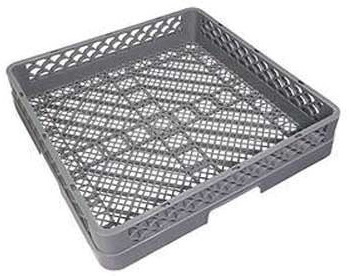
\includegraphics[height=6cm]{images/tray.jpg}
                \caption{Commercial Dishwashing Tray}\label{fig:tray}
            \end{figure}

            A gentry robot may be implemented to pick up the jars out of the tray to move them. The advantage of this style of robot is it is versatile and robust in it's actions. It can move anywhere within a predefined space, enough to encompass the entire tray and the conveyor ingress. The gantry is only a system of actuators and control systems, it still requires a subsystem to target where the jars are and thus where to move the end effector. 
            
            A camera may be implemented as a vision system for jar targeting. This can be used to sense the location of each jar present waiting to be unloaded, and pass the coordinates to the gantry robot.

        \subsection{Project Limitations}\label{sec:proj-limits}
            % needs to be on a rpi0. output meaningful for a targeting system.
            As per the project description, the processer hardware used must be a Raspberry Pi Zero W (hereafter ``Rpi''). This is single-board computer uses an ARMv6 architecture with a single-core CPU and no GPU. There is one available USB OTG connection. It has available and accessible GPIO and power pins. There is a connection for a CSI camera\cite{rpi}. 

            It was indicated in lecture that projects should include data collection via sensors connected to the Rpi as well as constructing the models. This greatly increases the project scope. Very large datasets are available  from open online sources. By using existing datasets, groups could have yielded interesting projects without needing to divert effort to anything other than than creating the models.

            Since the project is intended to be integrated into an existing workflow, the physical items involved must remain the same. This includes the tray and the jars. The jars could have been improved by coating the rim in a distinct colour easily discerned by the camera. The tray's bottom is a structure made of small crosses. The geometric complexity of the tray can cause issues for the model. 
            
            % TODO any other limitations? specific issue will be discussed later in methodology

        \subsection{Design Philosophy}
            As we are currently training as Mechatronic Systems Engineers, we opted to take a holistic system based approach. This meant splitting the project in discrete subsystems and focusing on the integrations between systems, including subsystems before and after the scope of this project. This allowed us to create a project which was easily integrated into the existing industrial system and process. 

            It was decided that data collection will be a crucial step in this project. Without a sufficient dataset to train with, no matter the quality of the model, the results will be poor. Garbage in, garbage out. Great effort was put into data collection and labelling.

            \textbf{Input}: An unencoded image from a camera of the jars in a tray.

            \textbf{Output}: A list of coordinates, a spatial map of jar locations, or a single jar's coordinates. %TODO keep whichever it is

    \FloatBarrier
    \section{Methodology}
        \subsection{Data Collection}
            The data collection and labelling was all done manually. A series of photos of jars in different configurations in a tray were taken and saved. Between each photo, one jar would be altered. Once Sufficient photos were taken, each would be manually labelled using a custom made GUI. The images and labels would then be stored in a database for use by a model in training.

            \subsubsection{Camera Frame}
                % physical frame the camera and pi are mounted on
                A physical frame was constructed from wood and spare parts which holds the Rpi and camera in a fixed location over the jars and tray. A picture may be seen in figure~\ref{fig:frame}. The red part on the arm is the Rpi and camera. This allowed pictures to be taken of a consistent angle containing the same proportion of the tray every time. If the photos were taken from different angles each time, there would be too many variables introduced. Doing this minimized the number of features the model would need to compute. The frame worked well and as intended.

                \begin{figure}[ht]
                    \centering
                    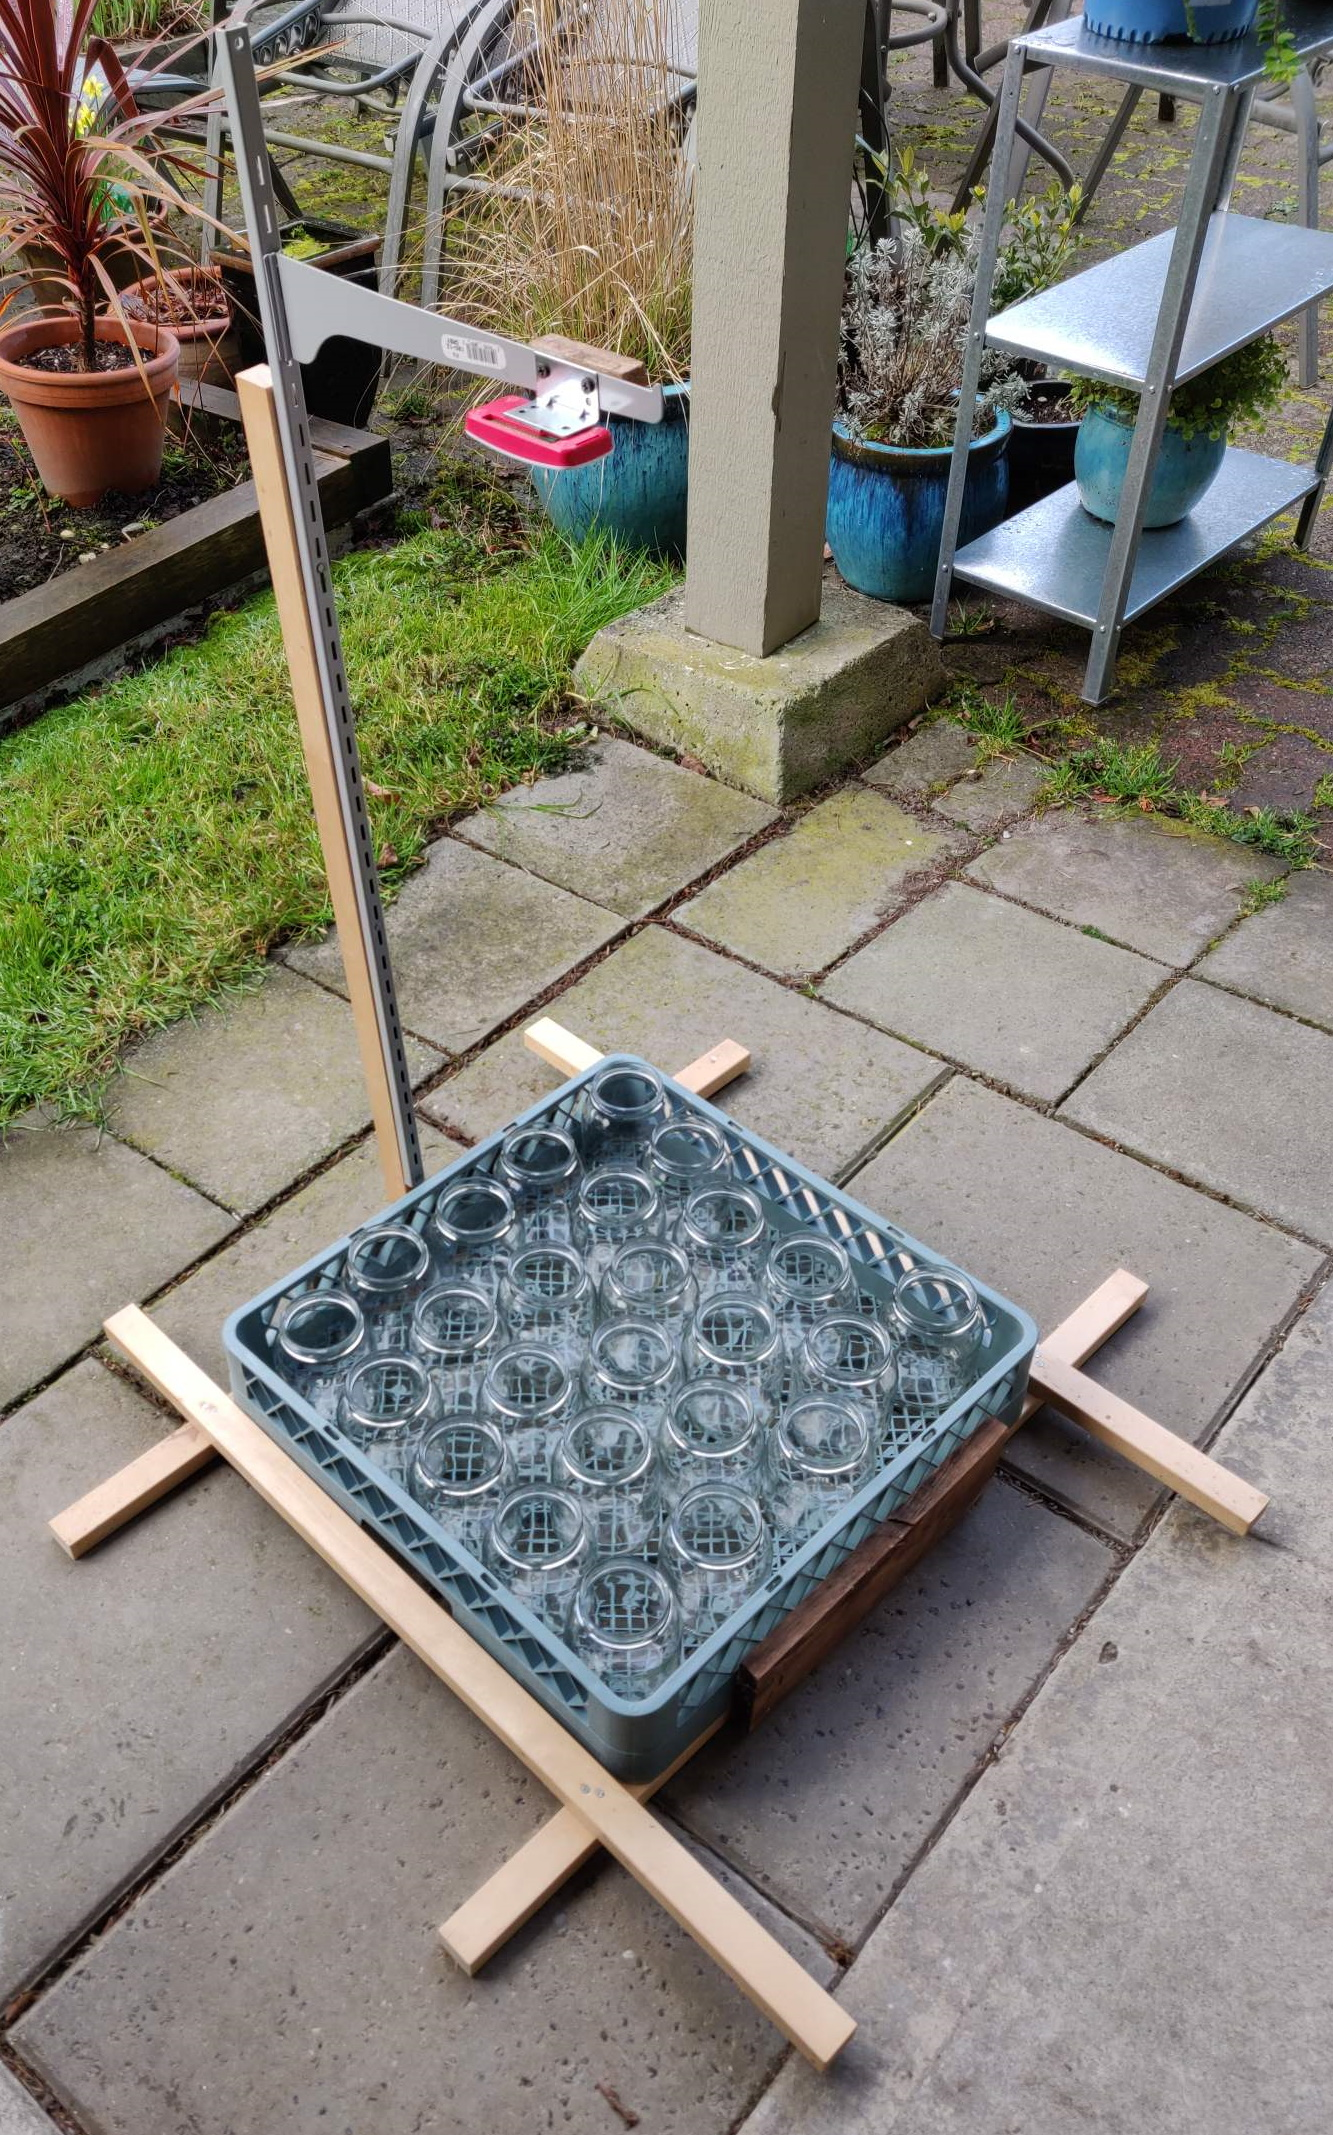
\includegraphics[height=9cm]{images/frame.jpg}      %TODO replace with better image
                    \caption{The Camera Mounting Frame}\label{fig:frame}
                \end{figure}

                The top-down perspective worked to mitigate the perspective warping from the camera lens. It will not be solved without a software transformation layer or the use of a different lens. It was decided that the perspective warping was outside the scope of this project.

            \subsubsection{Data Point Labelling}
                % taking photos and the GUI program
                To label the sizable collection of images collected with descript and precise coordinates, a program with a GUI was created. This program allowed fast labelling. A screenshot of this program may be seen in figure~\ref{fig:label-gui}. This program was exceedingly useful and greatly improved the data collection speed.

                % TODO
                \begin{figure}[ht]
                    \centering
                    
\includegraphics[height=9cm]{images/TODO.png}
                    \caption{The labelling program interface}\label{fig:label-gui}
                \end{figure}

                The interface was created with MatPlotLib, a graphing and visualization library for Python. To summarize how to use it, the user clicks on three points of the rim of a jar. A full user guide is present on the readme of the GitHub page~\cite{akkerman_hunter}. Using equations~\ref{eq:x_0} through~\ref{eq:r}, the centre and radius is determined mathematically.  \(M_{i,j}\) is the \((i,j)\) minor from linear algebra of a matrix of the points chosen by the user. The original math was described by Stephen R. Schmitt~\cite{schmitt}.

                \begin{align}
                    x_0 &= \frac{1}{2} \cdot \frac{M_{1,2}}{M_{1,1}} \label{eq:x_0}\\
                    y_0 &= -\frac{1}{2} \cdot \frac{M_{1,2}}{M_{1,1}} \label{eq:y_0}\\
                    r   &= x_0^2 + y_0^2 + \frac{M_{1,4}}{M_{1,1}} \label{eq:r}
                \end{align}

                There were issue in development with blocking inputs, sending interrupts from the buttons, and a memory leak. All of which were solved. After the images were labelled, the image, labels, and other information would be stored in a database.

            \subsubsection{Database Storage}
                % storing all the data points
                Given that our training data is images, the dataset had the potential to require massive amounts of storage and the surrounding infrastructure. Implementing a MySQL database was considered but opted against. The work required to initialise the container, expose it safely for us both work with it, and the additional learning required to integrate it with Python was deemed too great for the minimal benefits at our prospective scale. This would be a more future-proof solution, but was excessive for our use.

                What was used was simple a list of dictionaries pickled then compressed into several archive files. This is a normal means of small-scale data storage in Python. This gave us to advantages of each data point having several different types of data, all listed under their respective key. Using multiple archive files allowed pushing/uploading them to GitHub with only free accounts. Each data point contained the unencoded RGB image, a list of jar centre coordinates, the filename of the original
                
                Several compression methods were experimented with. Of those, Lempel–Ziv–Markov chain algorithm (LZMA) was found to preform the fastest. bzip2 was, unexpectedly, found to have the greatest compression, roughly 25\% better than LZMA but was slightly slower. Deflate was found to have no benefits over LZMA or bzip2. bzip2 was chosen because the speed was still acceptable along with the better compression.

        \subsection{Machine Learning Model}\label{sec:ml}
            % the Keras and other ML stuff
            \subsubsection{Data Augmentation}\label{sec:aug}
                % bolstering the data set with image transformations 
                Data augmentation is a technique used to bolster the training set without the need for additional data collection. There is built-in layers in Keras to preform augmentation of images via rotating, flipping, and cropping. This methods are intended for use in classification as they do not similarly transform the labels, so they were not valid for our use. Instead, we opted to design our own augmentation routine comprised only of flipping and rotating.

                By rotating each image to each of the four cardinal directions, and then flipping along four different axes, it would increase the amount of labelled data by a factor of 16. This, however, consumed a tremendous amount of memory in the process. More detail regarding memory may be found in section~\ref{sec:memory}. As a compromise, both rotations and flips were preformed, but not combined. This lead to a factor of 8 times increase in data while still remaining confined in available memory. Increasing the training data size greatly increased training time to a point where is is unfeasible to do so without a GPU.
                
            \subsubsection{Dataset Management}\label{sec:memory}
                % memory issues and types
                After the addition of data augmentation (section~\ref{sec:aug}), the far greater amount of data required a exorbitant amount of memory (RAM) to store. Initially, the input and label data were being stored as NumPy arrays. These have the disadvantage of needing to be stored entirely in RAM for the duration of their life. While using all permeations of data augmentation, Python would crash citing the need for an additional 19 GiB of memory. This was not feasible as no group member has such a computer. In an attempt to relegate the data to be stored on the disk (technically, a solid-state drive) rather than memory, a Tensor Flow Dataset was employed. 

                This type of dataset is designed for this exact purpose. It is possible to read the training data from the disk at the time of training and only enough for the batch being used. This method was not utilized to it's fullest, given time constraints. The possible prefetching or using the better memory managed TFRecord instead of NumPy arrays was not implemented. It was not exactly measured, but empirically it did seem to use less memory and more disk I/O after switching to the TF Dataset, indicating some level of caching on the disk was happening.

            \subsubsection{Base Model and Set-Up}
                The base model was found online, this model uses two hidden convolutional layers as well as the output being a convolutional layer~\cite{saif}. Unlike classification models, the output layer uses 'relu' as we are not looking for percentages of classifications, but actual locations of the jars. Glorot Normal was selected as is has become the standard initializer as it's performance was shown to be better through the truncated normal distribution, where the standard deviation is the the square root of two divided by the sum of input units in the tensor unit inputs and outputs. A unique loss function was created related to distance, as the desire of this model is to be able to predict locations. The loss function and therefore the distance between the model output and expected output will be minimized.
                % describing each layer in the model

            \subsubsection{Model Optimization Process}
                The initial model reported an accuracy in with highs of 70 to 80\%. Upon reviewing the output of the model, it was evident that even though native accuracy and loss metrics were implying a high performance model. The CNN was training itself to recognize and track the pattern and features of the jar tray instead of the jars themselves. The goal of optimizing our model was based around finding ways for the model to focus on the jars themselves.

                \paragraph{General Testing Process}
                    Due to the run-time required to train such a model, we applied technique of ``over stopping'', where the training is stopped when changes in the performance of the model starts to plateau, this was completed manually by observing when the reported accuracy value stopped changing, this was around 8 epochs. Through our research we learned that even though a higher batch size can increase the speed in which a model trains, a lower batch size can at times help the model converge, keeping this in mind, we kept the batch size at 32, the lowest standard batch size commonly used. This is similar to finding an elbow during k-value selection in Kmeans clustering, though the added complexity of training a model makes it difficult to automate in the same manner.

                \paragraph{Label Selection}
                    Initially, we tried using the method of labels discussed by Saif~\cite{saif} where the label was a series of points and the locations of the circles, or in our case: the jar openings. This was found to not converge very well, as the model was not able to find a relationship between the the open jars and a location. We then moved to creating our own image labels that contained circles of radius 35, which was found to be the average value found during the labelling process. Changing to this method made the jar shapes semi-noticeable in the the model output but it was not what the model was actually finding, as features of the tray were still much more distinct and noticeable to the model. 
                    
                    A possible solution of this was to change to the labels to be doughnut shapes, to better motivate the model to look for the edge that is the jar lip. Upon training, the accuracy reported was a false positive, as it was reporting accuracy in the 90s, but upon reviewing the results, it was found that the model's accuracy was only high as the output of the model was effectively blank. In the end, we determined that the best label was a fully filled-in circle with a radial gradient, with the outer edge of the circle being a lower value, progressively getting higher towards the centre. This allowed the model to focus on the full opening while still being sensitive to what we truly desired: the centre.

                \paragraph{Pooling Layers}
                    To reduce the sensitivity of the model to the jar opening vs. the tray, pooling was investigated to both try to potentially blur out the tray features, while also hopefully making the model more sensitive to the jar openings. First, average pooling was placed after the input layer and before the convolution layers to hopefully blur out the tray features, but this resulted in lower performance as the features of the tray were more distinct than those of the jars. In this attempt to blur out the tray, we blurred out the jars. After this, max and min pooling were applied in the same stages within the model. Max pooling is used to find the higher-value pixels whereas Min pooling is used to find the lower-value pixels. Both techniques were tested due to our inability to determine if the jars were darker or lighter than their surroundings. Min pooling is not an offered keras layer, so the images were first colour inverted, and then the max pooling function was used. Both max and min pooling were found to not be helpful for making the model more sensitive, as the jar colour was found to not be distinct enough from its surrounding pixels, so both pooling methods focused on features of the image that were more distinct than the jars. 

                \paragraph{Clustering for Preprocessing}
                    The next attempt to increase the distinctness of the jars was to apply k-means clustering to the input set before training the model. Different values of k were used on a test image and a k value of three was found to be the best in making the jars more distinct within the image. This proved to not be effective, as even though the clustering made the jars more noticeable to us, the previously mentioned fact that the colour of the jars was not distinct once again did not aid in the performance. The jars were clustered with other aspects of the images, which resulted in the jars themselves not standing out from the our portions of the cluster it was assigned to. Essentially what clustering did was reduce the full 24-bit RGB colour scheme to three discrete colours. The added run time was also a detriment. 

                \paragraph{Final Model Architecture}
                    During research, it was found that the best method to fine tune a model was to first over fit the model, then introduce techniques to generalize the model. This was attempted by adding an additional convolutional layer than the model introduced in the video~\cite{saif}. The accuracy change was negligible, so further convolutional layers were not added as the increase in performance was not worth the added time required to train a more complex model. Adding a dense layer was attempted to add more complexity to the model, but was not possible due to the memory required to have every node of the dense layer allocated to the parameters representing every pixel of the images. In the final model, a average pooling layer was place after the first convolutional layer to attempt to remove the features of the tray. 

        \subsection{Project Implementation and Integration}
            % how we got it to run on our hardware and how it will be integrated with the next subsystem
            \subsubsection{Tensor Flow on the Raspberry Pi}
                % how it got installed on armv6
                As mentioned in section~\ref{sec:proj-limits}, the Rpi uses ARMv6 architecture. This architecture is not officially supported by Tensor Flow (being 32-bit is fine). Using the standard pip install would not suffice and led to dependency issues or attempting unavailable processor instructions. Several methods were attempted to get a runtime installed on the Rpi which could run a model created using Keras. These including hunting a long list of dependencies and tracking down specific versions, attempting to compile from source, and using a myriad of outdated versions and prebuilt binaries. 
                
                The ultimate solution came in the form of a ``pip wheel'', a means of package distribution. It was created by GitHub user lhelontra~\cite{lontra}. This package successfully installed Tensor Flow 2.4 and the required dependencies and libraries onto the Rpi.

            \subsubsection{Exporting and Importing Models}
                % tflite model exporting/importing
                The model was trained on a more powerful desktop computer, as described in section~\ref{sec:ml}. The model then needed to be exported for use on the Rpi. Keras can directly save models. Another approach, which is what we used, is the TensorFlow Lite runtime library. This library is intended for this exact scenario, where a model is created elsewhere and then ran on a less powerful device. This worked well and allowed us to save a model from a desktop and run the inference on the Rpi with ease. If it TensorFlow was natively compatible with the Rpi, it is likely that only Tensor Flow Lite would need to be installed on the Rpi, rather than the entire Tensor Flow suite.

            \subsubsection{Raspberry Pi Program}
                % the program which executes on the pi. uses a pi camera to take and store photos for training. invokes the model when in use. full command line control possible.
                A Python program was written to run on the Rpi. The main purpose was to pass sensor information from the camera to the trained model to receive the jar coordinates \textbf{TODO} or whatever it is. The same program was also used to collect the data to be labelled for training. Unless specified otherwise, the program saves any new images so a human may label them at a later time. The program may be launched with specific settings by passing arguments in the command line. A full user guide may be found on our GitHub readme file~\cite{akkerman_hunter}.

            \subsubsection{Deriving Meaningful Data from the Model}
                % I don't know this yet. how the information is converted into something the robot can use.

    \FloatBarrier
    \section{Results}
        \subsection{Example Results}
            % pictures visualizing the output of sample data

        \subsection{Results Metrics}
            % measurements quantifying the results
    
    \FloatBarrier
    \section{Discussions}
        % lots of graphs

    \FloatBarrier
    \section{Conclusion}

    \FloatBarrier
    \section{Other}
        \subsection{Work Delegation}

    \FloatBarrier
    \appendix
    
	\bibliographystyle{IEEEtran}
	\bibliography{bib}\addcontentsline{toc}{section}{Referances}

	\section{List of Figures}
		\makeatletter
		\@starttoc{lof}% Print List of Figures
		\makeatother

	\section{List of Tables}
		\makeatletter
		\@starttoc{lot}% Print List of Tables
		\makeatother

\end{document}
